 \documentclass[paper=a4, fontsize=11pt]{scrartcl} % A4 paper and 11pt font size

\usepackage[T1]{fontenc} % Use 8-bit encoding that has 256 glyphs
\usepackage{fourier} % Use the Adobe Utopia font for the document - comment this line to return to the LaTeX default
\usepackage{amsmath,amsfonts,amsthm} % Math packages
\usepackage{braket}
\usepackage{lipsum} % Used for inserting dummy 'Lorem ipsum' text into the template

\usepackage{sectsty} % Allows customizing section commands
\allsectionsfont{\centering \normalfont\scshape} % Make all sections centered, the default font and small caps
\usepackage{pgfplots}
\usepackage{graphicx}


\usepackage{fancyhdr} % Custom headers and footers
\pagestyle{fancyplain} % Makes all pages in the document conform to the custom headers and footers
\fancyhead{} % No page header - if you want one, create it in the same way as the footers below
\fancyfoot[L]{} % Empty left footer
\fancyfoot[C]{} % Empty center footer
\fancyfoot[R]{\thepage} % Page numbering for right footer
\renewcommand{\headrulewidth}{0pt} % Remove header underlines
\renewcommand{\footrulewidth}{0pt} % Remove footer underlines
\setlength{\headheight}{13.6pt} % Customize the height of the header

\numberwithin{equation}{section} % Number equations within sections (i.e. 1.1, 1.2, 2.1, 2.2 instead of 1, 2, 3, 4)
\numberwithin{figure}{section} % Number figures within sections (i.e. 1.1, 1.2, 2.1, 2.2 instead of 1, 2, 3, 4)
\numberwithin{table}{section} % Number tables within sections (i.e. 1.1, 1.2, 2.1, 2.2 instead of 1, 2, 3, 4)

\setlength\parindent{0pt} % Removes all indentation from paragraphs - comment this line for an assignment with lots of text

%----------------------------------------------------------------------------------------
%	TITLE SECTION
%----------------------------------------------------------------------------------------

\newcommand{\horrule}[1]{\rule{\linewidth}{#1}} % Create horizontal rule command with 1 argument of height
\newcommand{\ketbra}[1]{\ket{#1}\bra{#1}}
\graphicspath {{./../Image/}}

\title{	
\normalfont \normalsize 
\horrule{0.5pt} \\[0.4cm] % Thin top horizontal rule
\huge Stats 441 - Homework 4 \\
\horrule{2pt} \\[0.5cm] % Thick bottom horizontal rule
}

\author{Junqiao Lin (20609800)} % Your name

\date{\normalsize\today} % Today's date or a custom date

\begin{document}

\maketitle % Print the title

%----------------------------------------------------------------------------------------
%	PROBLEM 1
%----------------------------------------------------------------------------------------

\newpage

\section*{Problem 1.}
a)

Note by definition, if $\hat{y} = 0$, we have
\begin{align*}
	P(y = 1) \Pi{j=1}^{n} P(x_j|y=1) &\leq P(y = 0) \Pi_{j=1}^{n} P(X_j|y=0) \\
	\log{\frac{P(y=1)}{P(y=0)}} + \Sigma_{j=1}^{n} \log(p(x_j|y=1)) - \log(p(x_j|y=0)) &\leq 0 \\
\end{align*}

Note since $x_j = 1$ we have $p(x_j|y=1) = P_{j1}$, $p(x_j|y=0) = P_{j0}$, $x_j = 0$ we have $p(x_j|y=1) = 1 - P_{j1}$, $p(x_j|y=0) = 1-P_{j0}$, thus we have:

\begin{align*}
\log{\frac{p}{1-p}} + \Sigma_{j=1}^{n} ((\log(p_{j1}) + \log(1 - p_{j0}) - \log(p_{j0}) - \log(1-p_{j0})) x_j +  (\log(1 - p_{j1}) - \log(1-p_{j0}))) &\leq 0 \\
 (\Sigma_{j=1}^{n} ((\log(p_{j1}) + \log(1 - p_{j0}) - \log(p_{j0}) - \log(1-p_{j0})) x_j) + (\Sigma_{j=1}^{n}  (\log(1 - p_{j1}) - \log(1-p_{j0}))) + \log{\frac{p}{1-p}}) &\leq 0
\end{align*}

Thus we have 
\begin{align*}
	w_j &= (\log(p_{j1}) + \log(1 - p_{j0}) - \log(p_{j0}) - \log(1-p_{j0})) \\
		&= \log(\frac{p_{j1} (1-p_{j0})}{(1-p_{j1})(p_{j0}) }) \\
	b   &= (\Sigma_{j=1}^{n}  (\log(1 - p_{j1}) - \log(1-p_{j0}))) + \log{\frac{p}{1-p}} \\
		&= \log(\frac{p}{1-p}\Pi_{i=1}^{n} \frac{1-p_{j1}}{1-p_{j0}} )
\end{align*}
\newpage
b) 

Note by definition, if $\hat{y} = 0$, we have
\begin{align*}
P(y = 1) \Pi{j=1}^{n} P(x_j|y=1) &\leq P(y = 0) \Pi_{j=1}^{n} P(X_j|y=0) \\
\log{\frac{P(y=1)}{P(y=0)}} + \Sigma_{j=1}^{n} (P(x_j|y=1) - \log(p(x_j|y=0))) &\leq 0 \\
\log{\frac{p}{1-p}} + \frac{1}{2}\Sigma_{j=1}^{n} ( \frac{(x_j - \mu_{j1})^2 - (x_j - \mu_{j0})^2 }{\sigma_j^2})  &\leq 0 \\
\log{\frac{p}{1-p}} + \frac{1}{2}\Sigma_{j=1}^{n} ( \frac{x_j^2 - 2x_j \mu_{j1} + \mu_{j1}^2 - x_j^2 + 2x_j \mu_{j0} - \mu_{j0}^2 }{\sigma_j^2})  &\leq 0 \\
\log{\frac{p}{1-p}} + \frac{1}{2}\Sigma_{j=1}^{n} ( \frac{- 2x_j \mu_{j1} + \mu_{j1}^2  + 2x_j \mu_{j0} - \mu_{j0}^2 }{\sigma_j^2})  &\leq 0 \\
\log{\frac{p}{1-p}} + \frac{1}{2}\Sigma_{j=1}^{n} ( \frac{(2 \mu_{j0} - 2\mu_{j1}) x_j}{\sigma_j^2} + \frac{\mu_{j1}^2  - \mu_{j0}^2 }{\sigma_j^2})  &\leq 0 \\
\Sigma_{j=1}^{n} ( \frac{(\mu_{j0} - \mu_{j1})}{\sigma_j^2})  x_j +  \Sigma_{j=1}^{n} (\frac{\mu_{j1}^2  - \mu_{j0}^2 }{2\sigma_j^2}) + \log{\frac{p}{1-p}}  &\leq 0 \\
\end{align*}


Thus we have 
\begin{align*}
w_j &= \frac{(\mu_{j0} - \mu_{j1})}{\sigma_j^2} \\
b   &= \Sigma_{j=1}^{n} (\frac{\mu_{j1}^2  - \mu_{j0}^2 }{2\sigma_j^2}) + \log{\frac{p}{1-p}}
\end{align*}
\newpage 

\section*{Problem 2.}
a) \\
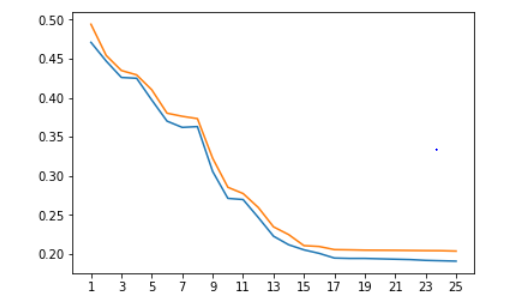
\includegraphics{A1I1} \\
Green: Training error \\
Yellow: Testing error \\
\\
c) The model seems to stabilize around $20\%$ and seems to never overfits after more iterations are added. It seems like using a stumps as the weak classifier reduces the chance of overfitting due to how inaccurate each individual stumps is to the model. 
\newpage

\section*{Problem 3.}
Note the LP problem is \\
$max_{\beta, \beta_0} \tau$, subject to $y_i(\beta^{T} x_i + \beta_0) \geq 1 \forall i$

Note since $\tau = \frac{1}{||\beta||}$, for $\beta,\beta_0$, we have $max_{\beta, \beta_0} \tau = min_{\beta, \beta_0} \frac{1}{\tau} = min_{\beta, \beta_0} ||B|| = min_{\beta, \beta_0} \frac{||B||^2}{2}$ 

Thus, by the Lagrangian we have
\begin{align*}
	L_p &= \frac{||\beta||^2}{2} + \Sigma_{i=1}^{n} \alpha_i [ y_i (\beta^{T} x_i + \beta_0) - 1 ] \\
	&= \frac{||\beta||^2}{2} + \Sigma_{i=1}^{n} \alpha_i y_i (\beta^{T} x_i + \beta_0) - \Sigma_{i=1}^{n} \alpha_i  \\
\end{align*}

After setting the derivative to zero we have \\
\begin{align*}
0 &=\beta - \Sigma_{i=1}^{n} \alpha_i  y_i x_i \\
\beta &= \Sigma_{i=1}^{n} \alpha_i  y_i x_i \\
\\
0 &= \Sigma_{i=1}^{n} \alpha_i  y_i
\end{align*}

Substituting the above into the Langrangian
\begin{align*}
0  &= \frac{||B||^2}{2} +  \frac{1}{2} \Sigma_{i=1}^{n} \alpha_i y_i (\Sigma_{j=1}^{n} \alpha_j  y_j x_j )x_i - \frac{1}{2}\alpha_i \\
\frac{||B||^2}{2} &=  \frac{1}{2} \Sigma_{i=1}^{n} \alpha_i -  \frac{1}{2} \Sigma_{i=1}^{n} \Sigma_{j=1}^{n}  \alpha_i \alpha_j  y_i y_j x_j x_i  \\
\frac{1}{\tau^2} &=  \Sigma_{i=1}^{n}\alpha_i -   \Sigma_{i=1}^{n} \Sigma_{j=1}^{n}  \alpha_i \alpha_j  y_i y_j x_j x_i  \\
\end{align*}

As desired



\end{document}